\sectionold{Вложенные структуры}

Теперь, как насчет ситуаций, когда одна структура определена внутри другой структуры?

\lstinputlisting{patterns/15_structs/5_nested/nested.c}

\dots в этом случае, оба поля \TT{inner\_struct} просто будут располагаться между полями a,b и d,e в 
\TT{outer\_struct}.

Компилируем (MSVC 2010):

\lstinputlisting[caption=\Optimizing MSVC 2010 /Ob0]{patterns/15_structs/5_nested/nested_msvc.asm}

Очень любопытный момент в том, что глядя на этот код на ассемблере, мы даже не видим, 
что была использована какая-то еще другая структура внутри этой!
Так что, пожалуй, можно сказать, что все вложенные структуры в итоге разворачиваются в одну, \IT{линейную} 
или \IT{одномерную} структуру.

Конечно, если заменить объявление \TT{struct inner\_struct c;} на \TT{struct inner\_struct *c;} 
(объявляя таким образом указатель), ситуация будет совсем иная.

% FIXME1: нарисовать вложенную структуру и развернутую

\clearpage
\subsectionold{\olly}
\myindex{\olly}

Загружаем пример в \olly и смотрим на 
\TT{outer\_struct} в памяти:

\begin{figure}[H]
\centering
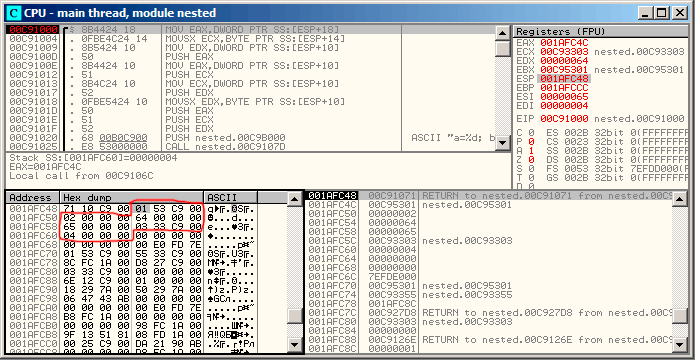
\includegraphics[scale=\FigScale]{patterns/15_structs/5_nested/olly.png}
\caption{\olly: Перед исполнением \printf}
\label{fig:nested_olly}
\end{figure}

Вот как расположены значения в памяти:
\begin{itemize}
\item \IT{(outer\_struct.a)} (байт) 1 + 3 байта случайного мусора;
\item \IT{(outer\_struct.b)} (32-битное слово) 2;
\item \IT{(inner\_struct.a)} (32-битное слово) 0x64 (100);
\item \IT{(inner\_struct.b)} (32-битное слово) 0x65 (101);
\item \IT{(outer\_struct.d)} (байт) 3 + 3 байта случайного мусора;
\item \IT{(outer\_struct.e)} (32-битное слово) 4.
\end{itemize}

